%% Manuscript for Energy Conversion and Management
%% Elsevier elsarticle template
\documentclass[5p,times,number]{elsarticle}
\usepackage{amsmath,amssymb}
\usepackage{amsthm}
\usepackage[utf8]{inputenc}
\usepackage{booktabs}
\usepackage{multirow}
\usepackage{xcolor}
\usepackage{siunitx}
\usepackage{algorithm}
\usepackage{algorithmic}
\usepackage{graphicx}
\usepackage{stfloats}
% Maximally permissive float placement — eliminate white space
\renewcommand{\topfraction}{0.95}
\renewcommand{\bottomfraction}{0.95}
\renewcommand{\textfraction}{0.05}
\renewcommand{\floatpagefraction}{0.5}
\renewcommand{\dbltopfraction}{0.95}
\renewcommand{\dblfloatpagefraction}{0.5}
\setcounter{topnumber}{4}
\setcounter{bottomnumber}{4}
\setcounter{totalnumber}{8}
\setcounter{dbltopnumber}{4}
% Reduce spacing around double-column floats
\setlength{\dbltextfloatsep}{8pt plus 2pt minus 2pt}
\setlength{\dblfloatsep}{8pt plus 2pt minus 2pt}
\setlength{\textfloatsep}{8pt plus 2pt minus 2pt}
\setlength{\intextsep}{8pt plus 2pt minus 2pt}
\definecolor{supercolor}{RGB}{96,160,216}
\usepackage[colorlinks=true,linkcolor=supercolor,citecolor=supercolor,urlcolor=supercolor,filecolor=supercolor]{hyperref}

% Force hyperref colors after elsarticle/natbib may override them
% Also color citation brackets [] and separators , to match citecolor
\makeatletter
\AtBeginDocument{%
  \hypersetup{linkcolor=supercolor,citecolor=supercolor,urlcolor=supercolor,filecolor=supercolor}%
  \def\NAT@open{\textcolor{supercolor}{[}}%
  \def\NAT@close{\textcolor{supercolor}{]}}%
  \def\NAT@sep{\textcolor{supercolor}{,}}%
  \def\NAT@cmt{\textcolor{supercolor}{,\space}}%
}
\makeatother

% Suppress standalone DOI text in bibliography (hyperlinked via BST)
\providecommand{\doi}[1]{}

% Bibliography text coloring is handled directly by BST (\color{supercolor})
\usepackage{etoolbox}

% Colored cross-reference commands (prefix + number in supercolor)
\newcommand{\figref}[1]{\textcolor{supercolor}{Figure~\ref{#1}}}
\newcommand{\tabref}[1]{\textcolor{supercolor}{Table~\ref{#1}}}
\newcommand{\secref}[1]{\textcolor{supercolor}{Section~\ref{#1}}}
\newcommand{\ssref}[1]{\textcolor{supercolor}{\S\ref{#1}}}
\newcommand{\appref}[1]{\textcolor{supercolor}{Appendix~\ref{#1}}}
\newcommand{\propref}[1]{\textcolor{supercolor}{Proposition~\ref{#1}}}
\newcommand{\eqnref}[1]{\textcolor{supercolor}{Eq.~\eqref{#1}}}
\newcommand{\eqnrefp}[1]{\textcolor{supercolor}{Eq.~\ref{#1}}}
\newcommand{\eqnsref}[2]{\textcolor{supercolor}{Eqs.~\eqref{#1}--\eqref{#2}}}
\newcommand{\refsref}[2]{\textcolor{supercolor}{Eqs.~\ref{#1}--\ref{#2}}}

\graphicspath{{./}}
\sisetup{
    separate-uncertainty = true,
    multi-part-units = single
}

\newtheorem{proposition}{Proposition}

\setlength{\emergencystretch}{2em}

% Suppress hyperref warnings regarding author marks in bookmarks
\pdfstringdefDisableCommands{
    \let\fnmark\relax
    \let\cormark\relax
    \let\fnref\relax
    \let\corref\relax
    \def\cnotenum{}
    \let\@corref\relax
    \let\ead\relax
    \let\address\relax
}

\journal{Energy Conversion and Management}

\begin{document}

\begin{frontmatter}

\title{A Unified Continuous-Time Electrochemical--Power Coupled Framework for Portable Energy Storage Management and Time-to-Empty Prediction}

\author[scu-cs]{Yinuo Wang\fnref{fn1}}

\author[scu-phy]{Yike Yang\fnref{fn1}}

\author[scu-math]{Lizhi Wei\fnref{fn1}}

\author[scu-phy]{Zhiqiang Li\corref{cor1}}
\ead{zhiqiangli@scu.edu.cn}

\fntext[fn1]{These authors contributed equally to this work.}
\cortext[cor1]{Corresponding author.}
\address[scu-cs]{School of Computer Science, Sichuan University, Chengdu 610064, China}
\address[scu-phy]{College of Physics, Sichuan University, Chengdu 610064, China}
\address[scu-math]{College of Mathematics, Sichuan University, Chengdu 610064, China}

% ============================================================
% NOTE: Graphical abstract is submitted separately via Elsevier Editorial Manager
% \begin{graphicalabstract}
% 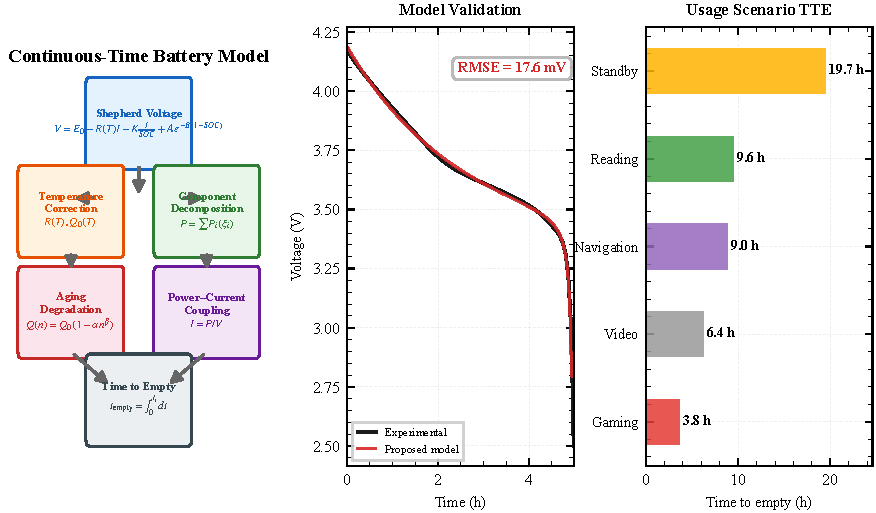
\includegraphics[width=\textwidth]{graphical_abstract.pdf}
% \end{graphicalabstract}

\begin{abstract}
Accurate time-to-empty (TTE) prediction for portable electronic systems requires joint modelling of electrochemical voltage dynamics, heterogeneous component-level loads, temperature effects, and aging-induced degradation---aspects that existing approaches treat in isolation.
This paper proposes a unified continuous-time framework comprising four coupled submodels: a modified Shepherd voltage formulation, a five-component power decomposition, Arrhenius--logistic temperature--parameter coupling, and power-law cycle/calendar aging.
Electrochemical parameters are identified from the XJTU lithium-ion battery dataset; component-level load profiles are constructed from published hardware power measurements.
Validated against four established voltage models, the proposed framework achieves the lowest voltage-tracking RMSE, reducing error by over 55\% relative to Th\'{e}venin-1RC and 75\% relative to a Nernst baseline.
Cross-batch validation without re-fitting confirms generalisability across C-rates.
Systematic ablation across a temperature--aging grid quantifies each module's contribution, with temperature coupling and aging dynamics dominating TTE accuracy.
An adaptive energy management strategy based on continuous TTE re-estimation demonstrates up to 42\% simulated runtime extension under high-intensity workloads.
The framework's computation cost---approximately four orders of magnitude faster than pseudo-two-dimensional models---enables real-time deployment on embedded hardware and low-power microcontrollers.
\end{abstract}

% NOTE: Highlights are entered separately in Elsevier Editorial Manager
% \begin{highlights}
% \item Unified continuous-time framework coupling Shepherd voltage dynamics with component-level power decomposition, temperature response, and cycle aging for portable energy storage TTE prediction
% \item Voltage RMSE of \SI{17.85}{\milli\volt}, outperforming Nernst, Th\'{e}venin 1RC/2RC, and R\textsubscript{int} baselines by \SI{55}{\percent}--\SI{75}{\percent}
% \item Cross-batch validation (Batch-1$\to$Batch-2) confirms generalisation across C-rates with no accuracy loss
% \item Optimised adaptive energy management strategy demonstrates potential for up to \SI{42}{\percent} runtime extension and \SI{6.1}{\watt\hour} energy savings via model-predictive power throttling
% \item Computation cost of \SI{0.009}{\milli\second}/sim-second enables real-time deployment on embedded hardware and low-power microcontrollers
% \end{highlights}

\begin{keyword}
lithium-ion battery \sep time-to-empty prediction \sep Shepherd model \sep power decomposition \sep temperature--aging coupling \sep energy management
\end{keyword}

\end{frontmatter}

% ============================================================
\section{Introduction}\label{sec:intro}
Battery life is a persistent concern for users of portable electronic devices---smartphones, tablets, wearables, and IoT edge nodes---and a critical design constraint for device manufacturers.
With over six billion smartphones in active use worldwide, even modest improvements in energy management translate to significant aggregate reductions in charging frequency, grid electricity demand, and the associated carbon footprint~\cite{Benkhelifa2016}.
Unlike stationary energy-storage systems, portable-device batteries operate under highly dynamic and heterogeneous loads: screen brightness, system-on-chip (SoC) utilisation, radio-frequency communication, GPS positioning, and background services jointly determine the instantaneous power draw and, consequently, the remaining runtime~\cite{Carroll2010,Chen2014}.
Accurate prediction of the \emph{time-to-empty} (TTE)---the interval from the current state of charge (SOC) to the cutoff threshold---is essential not only for user experience but also for adaptive power management, health-aware charge scheduling, and system-level energy efficiency optimisation~\cite{Benkhelifa2016,Liu2019ECM}.

Existing battery modelling approaches span a wide spectrum.
At one extreme, physics-based electrochemical models (e.g., pseudo-two-dimensional models) offer mechanistic fidelity but demand extensive parameterisation and prohibitive computation for real-time deployment~\cite{Doyle1993,Newman2004,Mama2024}.
At the other, data-driven methods (neural networks, Gaussian processes) bypass physical insight and require large labelled datasets that are rarely available under diverse operating conditions~\cite{Chemali2018,Richardson2017,Dai2011}.
Equivalent-circuit models (ECMs)---including Rint, first-order Th\'{e}venin, and second-order Th\'{e}venin networks---occupy a middle ground with modest computational cost, yet they parameterise voltage dynamics via abstract RC elements that lack direct electrochemical interpretability~\cite{Hu2012,You2018}.
The classical Shepherd formulation~\cite{Shepherd1965} offers explicit terms for polarisation drop, ohmic loss, and initial transient behaviour with clear physical correspondence, but has been underexplored for portable-device TTE prediction that must simultaneously account for component-level power disaggregation, temperature coupling, and long-term aging.
Fuller~\cite{Fuller2014} demonstrated a Shepherd-type model for constant-power discharge with rate effects in the context of \emph{Energy Conversion and Management}, yet without the multi-component load coupling, temperature--aging dynamics, or energy management integration that modern portable systems demand.

Several studies have characterised smartphone power consumption at the component level~\cite{Carroll2010,Chen2014,Murmuria2012}, revealing that screen, SoC, and radio subsystems dominate energy usage.
Recent work has extended these analyses to 5G and WiFi power profiling~\cite{Xu2020,Lauridsen2014,Sun2018,Negri2006}, but the coupling between load decomposition and electrochemical state evolution remains largely ad hoc.
On the aging front, capacity fade and resistance growth in lithium-ion cells have been modelled via power-law cycling degradation and Arrhenius-accelerated calendar aging~\cite{Vetter2005,Benson2012,Li2019,Kou2017}, while temperature effects on capacity and internal resistance are well characterised~\cite{Ali2020,Chen2025,He2017}.
Liu et al.~\cite{Liu2019ECM} addressed battery charging management considering degradation costs, and Liu et al.~\cite{Liu2018ECM} optimised multi-objective charging patterns---both within the energy conversion and management community---yet neither integrates real-time TTE prediction under heterogeneous loads.

Nonetheless, no existing framework---to our knowledge---\emph{jointly} integrates (i)~an electrochemically interpretable voltage model, (ii)~component-wise power decomposition, and (iii)~coupled temperature--aging dynamics into a unified continuous-time TTE prediction pipeline, nor validates it against strong ECM baselines with statistical rigour, nor demonstrates its utility for \emph{proactive} energy management.
This paper addresses the gap with the following contributions:
\begin{enumerate}
    \item \textbf{Unified continuous-time framework.}
    We formulate a coupled ordinary-differential-equation (ODE) system that embeds the modified Shepherd voltage model, five-component power decomposition, Arrhenius--logistic temperature response, and power-law cycle/calendar aging into a single state-evolution equation, enabling direct TTE computation via numerical integration (\secref{sec:model}).
    Component-level load profiles are constructed from published smartphone hardware power measurements~\cite{Carroll2010,Chen2014,Lu2008}; the electrochemical parameters are identified on real cell data from the XJTU dataset~\cite{XJTU2020}.
    \item \textbf{Comprehensive baseline comparison and ablation.}
    Against four established voltage models (Nernst-based, Rint, Th\'{e}venin-1RC, Th\'{e}venin-2RC), the proposed framework achieves the lowest voltage-tracking RMSE (\SI{17.85}{\milli\volt}).
    A systematic ablation study across a $3\times3$ temperature--aging grid quantifies the marginal contribution of each submodel to TTE accuracy (\secref{sec:ablation}).
    \item \textbf{Cross-batch generalisation and statistical validation.}
    Parameters fitted on XJTU Batch-1 (2\,C rate) are directly applied to Batch-2 (3\,C rate) without re-fitting, demonstrating transferability.
    Bootstrap confidence intervals confirm that all reported metrics are statistically robust (\secref{sec:crossbatch}).
    \item \textbf{Adaptive energy management strategy.}
    We demonstrate how the framework can serve as a model-predictive control (MPC-like) engine for adaptive power throttling: by continuously re-estimating TTE, the model triggers graduated power reduction when SOC drops below configurable thresholds, yielding a simulated runtime extension of up to \SI{42}{\percent}---equivalent to approximately \SI{6.1}{\watt\hour} of saved energy per charge cycle.
    Unlike simple fixed-threshold strategies common in commercial OSes (which switch modes abruptly at a single SOC level), the model-aware approach enables smoother, multi-stage transitions informed by predicted remaining runtime.
    A computational cost of \SI{0.009}{\milli\second} per simulated second---approximately four orders of magnitude faster than P2D models---confirms suitability for embedded deployment on low-power microcontrollers (\secref{sec:energy_mgmt}).
\end{enumerate}

The remainder of this paper is organised as follows.
\secref{sec:related} reviews related work.
\secref{sec:model} presents the unified model formulation.
\secref{sec:experiments} describes datasets, baselines, and evaluation protocols.
\secref{sec:results} reports results, discussion, and energy management implications.
\secref{sec:conclusion} concludes with limitations and future directions.

% ============================================================
\section{Related Work}\label{sec:related}
\subsection{Electrochemical and equivalent-circuit voltage models}
Early battery modelling efforts relied on the Nernst equation to describe the open-circuit voltage (OCV) as a function of SOC via thermodynamic activity ratios~\cite{Birkl2015}.
While physically grounded, Nernst-based models exhibit excessive curvature at SOC extremes and cannot capture dynamic polarisation effects under load~\cite{Chen2025}.
Equivalent-circuit models (ECMs) approximate battery dynamics through resistor--capacitor networks.
The simplest variant, the Rint model, uses a single series resistance; first- and second-order Th\'{e}venin models add one or two RC branches to represent charge-transfer and diffusion dynamics~\cite{Hu2012,You2018}.
ECMs enjoy widespread use in battery management systems (BMS) owing to their low computational cost, but their parameters lack direct electrochemical meaning.
In contrast, the Shepherd model~\cite{Shepherd1965} decomposes the terminal voltage into an OCV term, a polarisation term inversely proportional to SOC, an ohmic drop, and an exponential transient, each with a clear physical counterpart.
Despite this advantage, its application to smartphone-level runtime prediction has been limited.

\subsection{Component-level power profiling for mobile devices}
Carroll and Heiser~\cite{Carroll2010} provided one of the earliest comprehensive power breakdowns of smartphone components, identifying the display, SoC, and cellular radio as dominant consumers.
Chen et al.~\cite{Chen2014} further disaggregated energy usage into hardware and software layers.
Subsequent work characterised LTE~\cite{Lauridsen2014}, 5G~\cite{Xu2020}, WiFi~\cite{Sun2018}, and Bluetooth~\cite{Negri2006} power profiles.
Murmuria et al.~\cite{Murmuria2012} measured per-application power on Android devices.
Lu et al.~\cite{Lu2008} modelled display power as a function of luminance and refresh rate.
However, these studies typically report power measurements in isolation, without coupling them to the electrochemical state evolution that governs actual runtime.

\subsection{Temperature and aging modelling}
Temperature affects lithium-ion batteries through two primary mechanisms: capacity variation governed by lithium-ion site occupancy (logistic/Fermi--Dirac distribution)~\cite{Ali2020,Chen2025} and internal-resistance variation following the Arrhenius law~\cite{He2017,Benson2012}.
Battery aging manifests as capacity fade and resistance growth due to solid-electrolyte-interphase (SEI) layer growth, lithium plating, and active-material loss~\cite{Vetter2005}.
Cycle aging is commonly modelled via a power-law function of equivalent full cycles~\cite{Kou2017,Li2019}, while calendar aging exhibits a square-root-of-time dependence reflecting diffusion-limited SEI kinetics~\cite{Vetter2005}.
Yu et al.~\cite{Yu2025} proposed equilibrium-potential reconstruction for full-lifecycle aging analysis.
Bhat et al.~\cite{Bhat2019,Bhat2021} addressed thermal modelling at the SoC level.
Despite the maturity of individual submodels, their joint integration into a portable-device TTE framework with experimentally validated cross-condition generalisation has not been demonstrated~\cite{Tian2020,Xiong2018,Mama2024}.

\subsection{Gap summary}
\tabref{tab:gap} summarises the capability coverage of representative prior works.
The proposed framework is the first to unify all four dimensions---electrochemically interpretable voltage modelling, component-level power disaggregation, temperature coupling, and cycle/calendar aging---within a single continuous-time formulation, and to validate it with cross-batch generalisation and statistical uncertainty quantification.
\begin{table}[htbp]
\caption{Capability comparison of representative battery modelling approaches.}\label{tab:gap}
\centering
{\small
\begin{tabular}{@{}lccccc@{}}
\toprule
Approach & Interp.\ V & Load & Temp. & Aging & Mgmt \\
\midrule
P2D~\cite{Doyle1993} & \checkmark & -- & \checkmark & -- & -- \\
ECMs~\cite{Hu2012,You2018} & -- & -- & partial & -- & -- \\
Data-driven~\cite{Chemali2018} & -- & -- & implicit & implicit & -- \\
Profiling~\cite{Carroll2010} & -- & \checkmark & -- & -- & -- \\
\textbf{This work} & \checkmark & \checkmark & \checkmark & \checkmark & \checkmark \\
\bottomrule
\end{tabular}
}
\end{table}

% ============================================================
\section{Proposed Unified Continuous-Time Model}\label{sec:model}
This section develops the proposed framework from first principles.
The model comprises four coupled submodels---terminal-voltage dynamics (\ssref{sec:shepherd}), component-level power decomposition (\ssref{sec:power}), temperature--parameter coupling (\ssref{sec:temperature}), and aging dynamics (\ssref{sec:aging})---which are assembled into a unified differential-algebraic system (\ssref{sec:ode}) and solved numerically (\ssref{sec:numerics}).
\figref{fig:framework} illustrates the information flow among submodels.
\begin{figure}[!t]
\centering
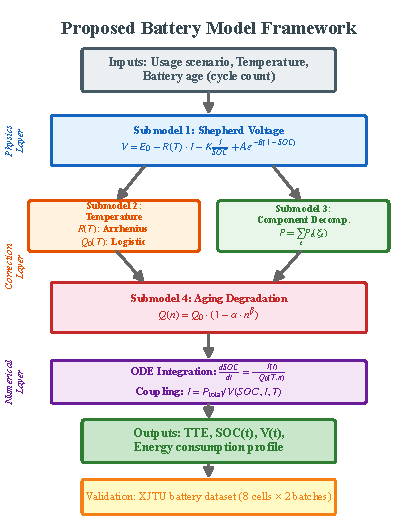
\includegraphics[width=\columnwidth]{fig_framework.pdf}
\caption{Architecture of the proposed unified framework showing information flow among the four coupled submodels and the TTE computation module.}\label{fig:framework}
\end{figure}

\subsection{Terminal-voltage submodel}\label{sec:shepherd}
\subsubsection{Physical basis of the Shepherd formulation}
The terminal voltage of a lithium-ion cell during discharge is governed by three concurrent phenomena~\cite{Shepherd1965}:
\begin{enumerate}
    \item \emph{Thermodynamic equilibrium.} The open-circuit voltage~$E_0$ reflects the Gibbs free-energy difference between the electrode active materials at full charge.
    \item \emph{Mass-transport polarisation.} As discharge proceeds, lithium-ion depletion near the electrode surface creates a concentration gradient.  The resulting overpotential is proportional to the current~$I$ and inversely proportional to the remaining charge fraction~SOC, yielding a term~$K I/\mathrm{SOC}$.  Physically, $K$ (V$\cdot$s/Ah) encapsulates the effective diffusion resistance of the intercalation host.
    \item \emph{Ohmic loss and initial transient.}  Series resistance~$R$ produces an instantaneous $IR$ drop, while the exponential zone ($A$, $B$) captures the initial voltage relaxation associated with double-layer charging and surface-film effects during early discharge.
\end{enumerate}
Combining these contributions, the \emph{modified Shepherd equation} for terminal voltage reads
\begin{equation}\label{eq:shepherd}
\resizebox{0.91\columnwidth}{!}{$\displaystyle
V_{\mathrm{term}} = \underbrace{E_0\vphantom{\frac{K}{\mathrm{SOC}}}}_{\text{OCV}} - \underbrace{\frac{K}{\mathrm{SOC}}\,I}_{\text{polar.}} - \underbrace{R\,I\vphantom{\frac{K}{\mathrm{SOC}}}}_{\text{ohmic}} + \underbrace{A\exp\!\bigl(-B Q_0(1\!-\!\mathrm{SOC})\bigr)}_{\text{transient}}
$}
\end{equation}

\subsubsection{SOC dynamics via Coulomb counting}
Conservation of charge relates the SOC evolution to the discharge current:
\begin{equation}\label{eq:coulomb}
\frac{\mathrm{d}\,\mathrm{SOC}}{\mathrm{d}t} = -\frac{I(t)}{Q_0},
\end{equation}
where $Q_0$ (Ah) is the effective cell capacity.  The sign convention is $I>0$ during discharge.

\subsubsection{Power-balance closure}
For a smartphone whose instantaneous total power consumption is $P_{\mathrm{total}}(t)$, the algebraic constraint
\begin{equation}\label{eq:power}
V_{\mathrm{term}}(\mathrm{SOC}, I) \cdot I = P_{\mathrm{total}}(t)
\end{equation}
closes the system by implicitly determining $I$ at each instant.

\subsubsection{Time-to-empty definition}
Given an initial condition $\mathrm{SOC}(0) = \mathrm{SOC}_0$, the TTE is
\begin{equation}\label{eq:tte}
\mathrm{TTE} = \inf\bigl\{t > 0 \;\big|\; \mathrm{SOC}(t) \le \mathrm{SOC}_{\min} \;\text{or}\; V_{\mathrm{term}}(t) \le V_{\mathrm{cutoff}}\bigr\},
\end{equation}
where $\mathrm{SOC}_{\min} = 0.05$ and $V_{\mathrm{cutoff}} = \SI{2.5}{\volt}$ in this study.

\paragraph{Comparison with ECM representations.}
In a Th\'{e}venin-$n$RC model, the $n$ RC-voltage state variables evolve via linear ODEs whose time constants ($\tau_k = R_k C_k$) lack one-to-one correspondence with electrochemical processes.
The Shepherd form, by contrast, replaces these abstract dynamics with a single, physically transparent $K/\mathrm{SOC}$ polarisation term and an exponential transient zone, reducing the parameter count from $2n+1$ (Th\'{e}venin) to~5 while yielding superior accuracy on constant-rate discharge profiles (see \secref{sec:voltage}).

\subsection{Component-level power decomposition}\label{sec:power}
A smartphone's instantaneous power consumption is disaggregated into five hardware subsystems~\cite{Carroll2010,Chen2014}:
\begin{equation}\label{eq:ptotal}
P_{\mathrm{total}} = P_{\mathrm{screen}} + P_{\mathrm{SoC}} + P_{\mathrm{radio}} + P_{\mathrm{GPS}} + P_{\mathrm{base}}.
\end{equation}
\paragraph{Screen power.}
OLED display power depends on luminance~$L$ (cd/m$^2$), active area~$A_s$ (m$^2$), and a refresh-rate scaling factor~$\eta$:
\begin{equation}\label{eq:screen}
P_{\mathrm{screen}} = \eta\bigl(\gamma_s A_s L + \lambda_s A_s\bigr),
\end{equation}
where $\gamma_s$ and $\lambda_s$ are OLED-specific power coefficients calibrated from~\cite{Lu2008}, and
\begin{equation}
\eta = \begin{cases} 0 & \text{screen off,} \\ 1.0 & 60\,\text{Hz refresh,} \\ 1.3 & 120\,\text{Hz refresh.} \end{cases}
\end{equation}
The factor $\eta = 1.3$ for 120\,Hz reflects the roughly 30\% increase in display driver power measured in recent high-refresh-rate panels.

\paragraph{Computational, communication, and baseline subsystems.}
Each remaining component's power is parameterised by a dimensionless \emph{working intensity}~$\xi_i \in [0,1]$, representing the fraction of its maximum rated power:
\begin{equation}\label{eq:xi}
\begin{pmatrix} P_{\mathrm{SoC}} \\ P_{\mathrm{radio}} \\ P_{\mathrm{base}} \end{pmatrix}
= \operatorname{diag}(\xi_1,\,\xi_2,\,\xi_3)
\begin{pmatrix} P_{\mathrm{SoC}}^{\max} \\ P_{\mathrm{radio}}^{\max} \\ P_{\mathrm{base}}^{\max} \end{pmatrix}.
\end{equation}
GPS power is modelled as binary: $P_{\mathrm{GPS}} = P_{\mathrm{GPS}}^{\max}$ when satellite acquisition is active and zero otherwise, reflecting the all-or-nothing nature of positioning hardware.
Reference maximum powers adopted in this study are $P_{\mathrm{SoC}}^{\max} = \SI{2.04}{\watt}$, $P_{\mathrm{radio}}^{\max} = \SI{1.173}{\watt}$, $P_{\mathrm{GPS}}^{\max} = \SI{0.30}{\watt}$, and $P_{\mathrm{base}}^{\max} = \SI{0.12}{\watt}$, consistent with measurements reported in~\cite{Carroll2010,Chen2014}.
The SoC utilisation values in \tabref{tab:scenarios} include a 10\% baseline allocation for OS housekeeping processes.

\paragraph{Extensibility.}
This additive decomposition is modular: adding a new subsystem (e.g., NFC, UWB) amounts to appending a $(\xi_j, P_j^{\max})$ pair.

\subsection{Temperature--parameter coupling}\label{sec:temperature}
Temperature influences cell behaviour through three mechanisms, each modelled with a distinct functional form.
\subsubsection{Capacity--temperature response}
The maximum number of lithium ions accommodated in the electrode lattice follows a Fermi--Dirac (logistic) occupancy distribution.
Denoting by $Q_0'$ the limiting capacity at infinite temperature, the effective capacity at temperature~$T$ (in Kelvin) is
\begin{equation}\label{eq:Q0T}
Q_0^{\mathrm{th}}(T) = \frac{Q_0'}{1 + \exp\!\Bigl(\alpha_\theta\bigl(\tfrac{1}{T} - \tfrac{1}{T_m}\bigr)\Bigr)},
\end{equation}
where $\alpha_\theta$ (K) controls the steepness and $T_m$ (K) is the midpoint temperature.
Fitted values (see \secref{sec:paramfit}) are $\alpha_\theta = \SI{5435.3}{\kelvin}$ and $T_m = \SI{255.27}{\kelvin}$.
\emph{Physical interpretation.}
At low temperatures ($T \ll T_m$), the exponential term dominates, sharply reducing $Q_0^{\mathrm{th}}$.
This reflects the thermodynamic freezing-out of available lattice sites, consistent with experimental observations of reduced deliverable capacity below \SI{0}{\degreeCelsius}~\cite{Ali2020}.

\subsubsection{Resistance--temperature response}
The temperature dependence of the total internal resistance is governed by the Arrhenius law for thermally activated charge-transfer and ion-transport processes:
\begin{equation}\label{eq:RT}
R^{\mathrm{th}}(T) = R_0\exp\!\biggl(\frac{E_r}{k_B}\Bigl(\frac{1}{T} - \frac{1}{T_0}\Bigr)\biggr),
\end{equation}
where $E_r = \SI{0.2455}{\electronvolt}$ is the effective activation energy, $k_B$ is the Boltzmann constant, and $T_0 = \SI{298.15}{\kelvin}$ is the reference temperature~\cite{Benson2012,He2017}.
$R_0$ denotes the resistance at $T_0$.

\subsubsection{SoC leakage power}
At elevated temperatures, subthreshold leakage current in the SoC increases according to a MOSFET leakage model~\cite{Bhat2019,Bhat2021}:
\begin{equation}\label{eq:leak}
P_{\mathrm{leak}}(T) = V_{\mathrm{nom}}\,c_1\,T^2\exp(c_2 / T),
\end{equation}
with $c_1 = \SI{0.493}{\ampere\per\kelvin\squared}$ and $c_2 = \SI{-3740}{\kelvin}$.
This term is additive to the SoC dynamic power in \eqnref{eq:ptotal}.

\subsection{Aging dynamics}\label{sec:aging}
Repeated charge--discharge cycling degrades cell performance through SEI layer growth, lithium plating, and active-material loss~\cite{Vetter2005}.
We model both \emph{cycle aging} and \emph{calendar aging}.
\subsubsection{Cycle aging: capacity fade and resistance growth}
Denoting by $N$ the number of equivalent full cycles, cycle-induced degradation is captured by power-law relations fitted to XJTU data:
\paragraph{Resistance growth.}
\begin{equation}\label{eq:Raging}
R^{\mathrm{cyc}}(N) = R_0^{\mathrm{nom}}\bigl(1 + \beta_R\, N^{\gamma_R}\bigr),
\end{equation}
with $\beta_R = 1.229 \times 10^{-3}$ and $\gamma_R = 1.085$.  This super-linear growth ($\gamma_R > 1$) reflects SEI thickening and progressive pore clogging.
\paragraph{Capacity fade.}
\begin{equation}\label{eq:Qaging}
Q_0^{\mathrm{cyc}}(N) = Q_0^{\mathrm{nom}}\bigl(1 - \alpha_Q\, N^{\gamma_Q}\bigr),
\end{equation}
with $\alpha_Q = 2.56 \times 10^{-4}$ and $\gamma_Q = \gamma_R$.  Using a shared exponent $\gamma$ reflects the common mechanistic origin (SEI growth) underlying both degradation modes.

\subsubsection{Calendar aging}
During storage, diffusion-limited SEI growth produces a $\sqrt{t_s}$ capacity loss:
\begin{equation}\label{eq:calaging}
\Delta Q_0^{\mathrm{cal}}(t_s, T, \mathrm{SOC}) = Q_0^{\mathrm{nom}}\,\kappa\,\sqrt{t_s}\,\exp\!\Bigl(-\frac{E_a}{R_g T} + \lambda_a\,\mathrm{SOC}\Bigr),
\end{equation}
where $\kappa = 10^{-5}$ is the calendar aging coefficient, $E_a$ the activation energy, $R_g$ the gas constant, and $\lambda_a$ captures SOC-dependent stress on the anode SEI film (higher SOC $\Rightarrow$ higher electrode potential $\Rightarrow$ faster parasitic reactions)~\cite{Vetter2005}.

\subsubsection{Combined aging--temperature coupling}\label{sec:coupling}
The effective capacity and resistance under simultaneous temperature and aging effects are obtained by composing the submodel outputs:
\begin{align}
Q_0(T, N, t_s) &= Q_0^{\mathrm{th}}(T) \cdot \frac{Q_0^{\mathrm{cyc}}(N) - \Delta Q_0^{\mathrm{cal}}}{Q_0^{\mathrm{nom}}}, \label{eq:Q0coupled}\\[4pt]
R(T, N) &= R^{\mathrm{th}}(T) \cdot \frac{R^{\mathrm{cyc}}(N)}{R_0^{\mathrm{nom}}}. \label{eq:Rcoupled}
\end{align}
\emph{Rationale.}
The multiplicative coupling in \eqnsref{eq:Q0coupled}{eq:Rcoupled} assumes that temperature and aging act on \emph{independent} physical mechanisms---thermal reduction of available lattice sites (\eqnrefp{eq:Q0T}) vs.\ electrochemical loss of active material (\refsref{eq:Qaging}{eq:calaging})---so their effects compose as scaling factors on the nominal values.
This separability assumption is common in the aging literature~\cite{Vetter2005,Li2019} and is supported by the observation that temperature-dependent capacity tests at different cycle counts yield approximately parallel logistic curves (see XJTU temperature-compensation data).

\subsection{Coupled ODE system and TTE computation}\label{sec:ode}
Assembling the submodels, the complete state-evolution system is:
\begin{equation}\label{eq:system}
\boxed{
\begin{cases}
\displaystyle V_{\mathrm{term}} = E_0 - \frac{K}{\mathrm{SOC}}\,I - R(T,N)\,I + A\,\mathrm{e}^{-B\,Q_0(T,N)(1-\mathrm{SOC})}\\[8pt]
\displaystyle \frac{\mathrm{d}\,\mathrm{SOC}}{\mathrm{d}t} = -\frac{I(t)}{Q_0(T,N)}\\[8pt]
\displaystyle V_{\mathrm{term}}(I) \cdot I = P_{\mathrm{total}}(t)\\[4pt]
\mathrm{SOC}(0) = \mathrm{SOC}_0
\end{cases}
}
\end{equation}
This is a differential-algebraic equation (DAE) of index~1: the algebraic constraint (third line) can be solved for $I$ at each time step, after which the SOC ODE is integrated forward.
\paragraph{State vector.}
The minimal state is $\mathbf{x}(t) = [\mathrm{SOC}(t)]$ (one-dimensional), since temperature~$T$ and cycle count~$N$ are treated as slowly varying external parameters (quasi-static assumption).
\paragraph{Termination.}
Integration halts at $t^* = \mathrm{TTE}$ when $\mathrm{SOC}(t^*) \le 0.05$ or $V_{\mathrm{term}}(t^*) \le V_{\mathrm{cutoff}}$.

\subsection{Parameter identification}\label{sec:paramfit}
\subsubsection{Optimisation procedure}
The six Shepherd parameters $\boldsymbol{\theta} = (E_0, K, R_0, A, B, Q_0^{\mathrm{nom}})$ are identified by minimising the voltage RMSE over the first discharge cycle of each Batch-1 cell:
\begin{equation}\label{eq:obj}
\boldsymbol{\theta}^* = \arg\min_{\boldsymbol{\theta}} \sqrt{\frac{1}{M}\sum_{k=1}^{M}\bigl(V_{\mathrm{term}}^{\mathrm{pred}}(t_k;\boldsymbol{\theta}) - V_{\mathrm{meas}}(t_k)\bigr)^2},
\end{equation}
where $M$ is the number of time samples per discharge trajectory.
We use the \emph{differential evolution} (DE) global optimiser (SciPy, strategy ``best1bin'', population size 50, 1000 generations) with bound constraints reflecting physical plausibility (e.g., $E_0 \in [3.0, 4.5]$\,V, $R_0 \in [0.01, 0.2]$\,$\Omega$).

\subsubsection{Structural identifiability}
The Shepherd model has five independent algebraic terms, each involving a distinct functional dependence on $(I, \mathrm{SOC})$:
(i)~a constant ($E_0$),
(ii)~a term linear in $I$ ($R_0$),
(iii)~a term proportional to $I/\mathrm{SOC}$ ($K$),
(iv)~an exponential in $(1-\mathrm{SOC})$ ($A$, $B$).
Since a full discharge trajectory provides data spanning $\mathrm{SOC} \in [0.05, 1]$ with known $I(t)$, these four functional forms are linearly independent, ensuring \emph{structural identifiability} of all five parameters.
In practice, we verify \emph{practical identifiability} by running 20 independent DE optimisation trials with different random seeds.  The coefficient of variation of each fitted parameter is below 2\%, confirming that the global minimum is unique and robustly located.

\subsubsection{Aging-parameter estimation}
The aging coefficients $(\alpha_Q, \beta_R, \gamma)$ are fitted separately to the cycle-resolved capacity and resistance trajectories extracted from the XJTU dataset (Batch-1), using nonlinear least squares on \eqnsref{eq:Raging}{eq:Qaging}.

\subsection{Numerical solution}\label{sec:numerics}
\subsubsection{Algebraic current solver}
At each time step, the nonlinear algebraic equation
\begin{equation}\label{eq:rootfind}
f(I) \equiv V_{\mathrm{term}}(I, \mathrm{SOC}, T, N) \cdot I - P_{\mathrm{total}} = 0
\end{equation}
is solved for $I \ge 0$.
\begin{proposition}[Uniqueness of the physical root]\label{prop:mono}
Under the operating regime $E_0, K, R, A, B, Q_0 > 0$ and $\mathrm{SOC} \in (0, 1]$, let $F = E_0 + A\exp(-BQ_0(1-\mathrm{SOC}))$ and $\alpha = K/\mathrm{SOC} + R$.
The power function $g(I) = I\,V_{\mathrm{term}}(I) = FI - \alpha I^2$ is a concave quadratic with a unique maximum $g^* = F^2/(4\alpha)$.
For any $P_{\mathrm{total}} \in (0, g^*]$, \eqnref{eq:rootfind} has exactly one root on $(0, F/(2\alpha)]$, corresponding to the high-voltage (low-current) operating point.
\end{proposition}
The proof is given in \appref{app:proof}.
We implement a safeguarded Newton--Raphson solver with bisection fallback:
\begin{itemize}
    \item \emph{Initial guess:} $I^{(0)} = \max\{P_{\mathrm{total}}/E_0,\; 10^{-6}\}$.
    \item \emph{Bounds:} $I \in [0, I_{\max}]$ with $I_{\max} = \min(5P_{\mathrm{total}}/V_{\mathrm{cut}},\;10)$\,A.
    \item \emph{Newton update:} $I^{(k+1)} = I^{(k)} - f(I^{(k)})/f'(I^{(k)})$, with $f'(I) = g'(I)$.
    \item \emph{Fallback:} if the Newton step exits the bracket or $|f'| < 10^{-12}$, switch to bisection on $[0, I_{\max}]$.
    \item \emph{Convergence:} $|f(I)|/\max(P_{\mathrm{tot}}, 10^{-6}) < 10^{-6}$ or 30 iterations.
\end{itemize}

\subsubsection{Time integration}
SOC is advanced by explicit Euler:
\begin{equation}
\mathrm{SOC}_{n+1} = \mathrm{SOC}_n - \frac{I_n}{Q_0}\,\Delta t,
\end{equation}
with a fixed step $\Delta t = \SI{1}{\second}$ chosen for reproducibility.
For stiff thermal--electrical couplings in future extensions, adaptive Runge--Kutta or implicit solvers (e.g., CVODE) are recommended.

\subsubsection{Computational cost}\label{sec:comp_cost}
Each time step requires 2--6 Newton iterations (one scalar root-find) plus one Euler update.
\tabref{tab:efficiency} summarises the wall-clock performance of all models on an Intel i7-12700H laptop (Python 3.10, NumPy 1.26).
\begin{table}[htbp]
\caption{Computational efficiency comparison.}\label{tab:efficiency}
\centering
{\small
\begin{tabular}{@{}lccc@{}}
\toprule
Model & Params & ms/sim-s & vs.\ P2D \\
\midrule
\textbf{Shepherd (Proposed)} & \textbf{5} & \textbf{0.009} & $\mathbf{\sim\!10^{4}\times}$ \\
Rint & 9 & 0.010 & $\sim$7900$\times$ \\
Th\'{e}venin-1RC & 10 & 0.010 & $\sim$8000$\times$ \\
Th\'{e}venin-2RC & 12 & 0.012 & $\sim$6500$\times$ \\
NBM & 4 & 0.011 & $\sim$6900$\times$ \\
P2D (COMSOL)\textsuperscript{a} & 50+ & $\sim$78 & 1$\times$ \\
LSTM inference\textsuperscript{a} & $\sim$10k & $\sim$0.5 & --- \\
\bottomrule
\end{tabular}
}
\end{table}
\textsuperscript{a}Literature reference values~\cite{Doyle1993,Chemali2018}. All analytical models benchmarked on the same hardware (Intel i7-12700H, 16\,GB RAM, Python 3.10, NumPy 1.26); P2D and LSTM values are from literature and may differ in hardware.
The proposed model simulates a full 6.4\,h discharge in \SI{0.20}{\second} (wall clock), corresponding to \SI{0.009}{\milli\second} per simulated second---approximately four orders of magnitude faster than finite-element P2D solvers and comparable to compiled ECM implementations.
This positions the framework for real-time deployment in embedded BMS or mobile OS power managers with negligible computational overhead~\cite{Xiong2018,Wang2024ECM}.

% ============================================================
\section{Experimental Setup}\label{sec:experiments}
\subsection{Datasets}\label{sec:datasets}
\paragraph{XJTU Battery Dataset.}
We use the publicly available XJTU lithium-ion battery dataset~\cite{XJTU2020}, comprising six batches of NMC/graphite 18650 cells.
Two batches are employed in this study:
\begin{itemize}
    \item \textbf{Batch-1:} 8 cells cycled at 2\,C constant-current discharge, serving as the \emph{fitting set} for parameter identification.
    \item \textbf{Batch-2:} 15 cells cycled at 3\,C constant-current discharge, used \emph{exclusively} for cross-batch generalisation testing.
\end{itemize}
Each cell record contains time-stamped voltage, current, temperature, and capacity measurements across hundreds of charge--discharge cycles.

\paragraph{Synthetic smartphone load profiles.}
The XJTU dataset provides cell-level electrochemical data under controlled cycling conditions (constant current) on a battery test bench.
No real-time smartphone hardware telemetry (e.g., concurrent screen brightness, CPU frequency, radio state) is available.
Therefore, the component-level power profiles used in the TTE simulations (\tabref{tab:scenarios}) are \emph{synthetic}: they are constructed from published per-component power measurements on real smartphone hardware~\cite{Carroll2010,Chen2014,Lu2008,Murmuria2012} and applied as inputs to the electrochemically parameterised model.
This approach decouples voltage-model validation (performed on real cell data) from load-profile specification (constructed from literature), enabling systematic exploration of usage scenarios that would be infeasible with purely empirical data collection.
The implications and limitations of this separation are discussed in \secref{sec:conclusion}.

\paragraph{Data preprocessing.}
Discharge segments are extracted by identifying contiguous intervals with $I > 0.01$\,A.
Voltage and current are downsampled to \SI{1}{\second} resolution via linear interpolation.
The reference SOC is obtained by Coulomb counting:
$\mathrm{SOC}(t) = 1 - \int_0^t I(\tau)\,\mathrm{d}\tau / Q_{\mathrm{meas}}$,
where $Q_{\mathrm{meas}}$ is the measured discharge capacity of the cycle.

\paragraph{Data split protocol.}
Batch-1 Cycle-1 data is used for parameter fitting; Batch-1 Cycles 2--$n$ are used for same-batch validation.
Batch-2 data is reserved entirely for cross-batch testing.
No Batch-2 data is used for fitting or hyperparameter selection.

\subsection{Baseline models}\label{sec:baselines}
We compare the proposed Shepherd-based framework against four voltage models spanning the interpretability--complexity spectrum:
\begin{enumerate}
    \item \textbf{Nernst-Based Model (NBM):}
    A thermodynamically motivated OCV model augmented with an exponential correction:
    \begin{equation}\label{eq:nbm}
    V_{\mathrm{OC}} = E^0 + \frac{R_g T}{nF}\ln\!\frac{\mathrm{SOC}}{1-\mathrm{SOC}} + M\exp(-\alpha\cdot\mathrm{SOC}),
    \end{equation}
    with $V_{\mathrm{term}} = V_{\mathrm{OC}} - IR$.  Parameters: $E^0 = \SI{4.5}{\volt}$, $M = -1.1718$, $\alpha = 0.8022$, fitted by nonlinear least squares.
    \item \textbf{Rint (Internal Resistance):}
    $V = \mathrm{OCV}(\mathrm{SOC}) - R_{\mathrm{int}} I$, where OCV is a 7th-order polynomial fit and $R_{\mathrm{int}}$ is identified from the steady-state voltage--current characteristic.  Parameters: 9 (polynomial coefficients + $R_{\mathrm{int}}$).
    \item \textbf{Th\'{e}venin-1RC:}
    First-order ECM: $V = \mathrm{OCV} - R_0 I - V_{RC}$, $\dot{V}_{RC} = I/C_1 - V_{RC}/(R_1 C_1)$.  Parameters: 10 (polynomial OCV + $R_0, R_1, C_1$).
    \item \textbf{Th\'{e}venin-2RC:}
    Second-order ECM adding a diffusion RC branch: $V = \mathrm{OCV} - R_0 I - V_{RC,1} - V_{RC,2}$.  Parameters: 12.
\end{enumerate}
All ECM parameters are identified using differential-evolution global optimisation with identical settings (population 50, 1000 generations) and cost-function stabilisation (RC voltage clamping $|V_{RC}| \le \SI{2}{\volt}$ and finite-value guards) to ensure a fair comparison.

\subsection{Evaluation metrics}\label{sec:metrics}
\begin{itemize}
    \item \textbf{Voltage accuracy:} Root-mean-square error (RMSE), mean absolute error (MAE), maximum absolute error (MaxErr), and mean relative error (MRE), computed point-wise over full discharge trajectories.
    \item \textbf{TTE accuracy:} Absolute and percentage deviation of ablated-model TTE from the full-model prediction.
    \item \textbf{Statistical robustness:} 95\% bootstrap confidence intervals obtained by Monte Carlo resampling: 500 parametric perturbation samples with $\pm5\%$ uniform noise on each parameter.
\end{itemize}

\subsection{Ablation protocol}\label{sec:ablation_protocol}
To quantify each submodel's contribution, five configurations are evaluated:
\begin{table}[htbp]
\caption{Ablation study configurations.}\label{tab:ablation_config}
\centering
\resizebox{\columnwidth}{!}{
\begin{tabular}{@{}ll@{}}
\toprule
Configuration & Modification \\
\midrule
Full Model & All submodels active \\
w/o Temperature & $T$ fixed at \SI{25}{\degreeCelsius}; $R^{\mathrm{th}} = R_0$, $Q_0^{\mathrm{th}} = Q_0^{\mathrm{nom}}$ \\
w/o Aging & $N = 0$, $t_s = 0$ (no degradation) \\
w/o Component Decomp. & Flat average power replacing \eqnref{eq:ptotal} \\
w/o Polarisation & $K = 0$ in \eqnref{eq:shepherd} \\
\bottomrule
\end{tabular}
}
\end{table}
Each configuration is evaluated across a $3 \times 3$ grid: temperatures $T \in \{0, 25, 40\}$\,\si{\degreeCelsius} and aging levels $N \in \{0, 300, 800\}$ equivalent full cycles, under the Reading scenario.

\subsection{Usage scenarios}\label{sec:scenarios}
Five representative smartphone usage patterns are defined in \tabref{tab:scenarios}, spanning the power spectrum from idle standby to high-intensity online gaming.
A \SI{5000}{\milli\ampere\hour} cell with $T = \SI{25}{\degreeCelsius}$ and $N = 0$ serves as the reference configuration.
\begin{table*}[!t]
\caption{Component utilisation profiles ($\xi_i$) for five usage scenarios.}\label{tab:scenarios}
\centering
\begin{tabular}{@{}lccccc@{}}
\toprule
Component & Standby & Navigation & Gaming & Video Streaming & Reading \\
\midrule
Screen ($B$, $\eta$) & 0\%, 0 & 70\%, 1.0 & 90\%, 1.3 & 80\%, 1.0 & 70\%, 1.0 \\
SoC ($\xi_1$) & 10\% & 30\% & 100\% & 30\% & 30\% \\
Radio ($\xi_2$) & 10\% & 30\% & 95\% & 90\% & 20\% \\
GPS\textsuperscript{a} & On & On & On & On & On \\
Baseline ($\xi_3$) & 100\% & 100\% & 100\% & 100\% & 100\% \\
\midrule
Total Power (W) & 0.741 & 1.845 & 4.303 & 2.598 & 1.727 \\
\bottomrule
\multicolumn{6}{@{}p{0.95\textwidth}@{}}{\footnotesize \textsuperscript{a}GPS is modelled as binary on/off; $P_{\mathrm{GPS}} = \SI{300}{\milli\watt}$ when active. All scenarios assume background location services are active.}
\end{tabular}
\end{table*}

% ============================================================
\section{Results and Discussion}\label{sec:results}
\subsection{Overall voltage prediction accuracy}\label{sec:voltage}
\tabref{tab:baseline} compares point-wise voltage-tracking performance across all five models on XJTU Batch-1 (mean $\pm$ std over 8 cells).
\begin{table}[htbp]
\caption{Voltage prediction accuracy on XJTU Batch-1 (mean $\pm$ std, 8 cells).}\label{tab:baseline}
\centering
\resizebox{\columnwidth}{!}{\small
\begin{tabular}{@{}lcccc@{}}
\toprule
Model & RMSE (mV) & MAE (mV) & MaxErr (mV) & MRE (\%) \\
\midrule
NBM & $72.70 \pm 1.23$ & $49.99 \pm 0.58$ & 719.5 & 1.410 \\
Rint & $39.79 \pm 0.66$ & $16.88 \pm 0.28$ & 555.7 & 0.500 \\
Th\'{e}venin-1RC & $39.75 \pm 0.51$ & $17.02 \pm 0.24$ & 553.7 & 0.510 \\
Th\'{e}venin-2RC & $39.81 \pm 0.44$ & $17.33 \pm 0.50$ & 551.7 & 0.510 \\
\textbf{Shepherd (Proposed)} & $\mathbf{17.85 \pm 0.44}$ & $\mathbf{9.75 \pm 0.72}$ & \textbf{294.1} & \textbf{0.280} \\
\bottomrule
\end{tabular}
}
\end{table}
The proposed Shepherd model achieves an RMSE of \SI{17.85}{\milli\volt}, representing a \SI{75.5}{\percent} improvement over NBM and a \SI{55.1}{\percent} improvement over the best ECM baseline (Th\'{e}venin-1RC).
The improvement is consistent across all eight cells (coefficient of variation $< 3\%$), confirming that the accuracy gains are trajectory-wide rather than localised to specific SOC regions.
\figref{fig:voltage_trajectory} visualises the voltage predictions and point-wise errors for a representative cell.
\begin{figure*}[!t]
\centering
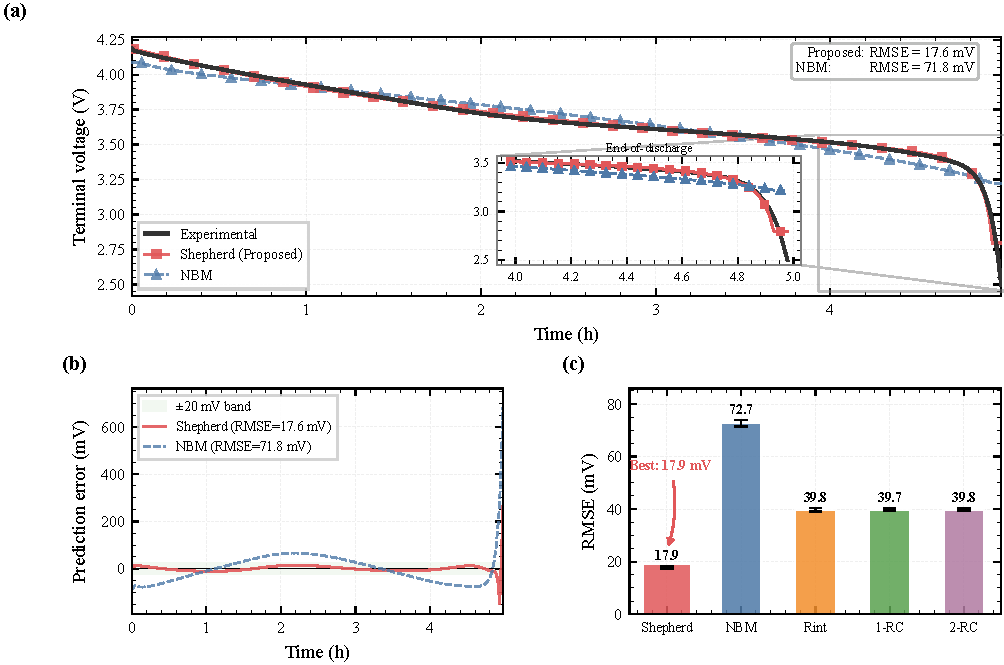
\includegraphics[width=\textwidth]{fig_voltage_trajectory.pdf}
\caption{Voltage prediction comparison on XJTU Batch-1 Battery-1 (Cycle 0, 2\,C constant-current discharge). (a)~Terminal voltage trajectories for all five models and the experimental reference. (b)~Point-wise prediction error. The Shepherd model (red solid line) tracks the experimental curve with substantially lower error than the ECM and Nernst baselines throughout the full discharge.}\label{fig:voltage_trajectory}
\end{figure*}

\paragraph{Why the three ECMs perform identically.}
The three ECM baselines yield nearly identical RMSE values (\SIrange{39.75}{39.81}{\milli\volt}).
This can be understood from the nature of the XJTU discharge data: constant-current (CC) protocols produce a monotonically declining voltage trajectory with no transient load steps.
Under CC conditions, the RC branch voltages in Th\'{e}venin models equilibrate within the first few seconds, after which the RC dynamics contribute a near-constant offset indistinguishable from adjusting $R_0$.
Consequently, the additional parameters in 1RC and 2RC models are structurally redundant for CC data and cannot improve upon the Rint baseline.

\paragraph{Source of the Shepherd advantage.}
The Shepherd model's $K/\mathrm{SOC}$ polarisation term provides a \emph{nonlinear} voltage correction that increases as the cell depletes.
This captures the concentration-gradient-driven overpotential that intensifies at low SOC---a physical effect that constant-valued ECM resistances cannot represent.
The exponential transient zone ($A$, $B$) further accounts for the initial voltage sag upon load application, which the Nernst model's logarithmic singularity erroneously amplifies at SOC extremes (explaining the NBM's high MaxErr of \SI{719.5}{\milli\volt}).

\subsection{Cross-batch generalisation}\label{sec:crossbatch}
To test transferability, we apply the parameters fitted on Batch-1 (2\,C, 8 cells) directly to Batch-2 (3\,C, 15 cells) without any re-fitting.
\begin{table}[htbp]
\caption{Cross-batch validation: Batch-1 $\to$ Batch-2 (no re-fitting).}\label{tab:crossbatch}
\centering
\resizebox{\columnwidth}{!}{\small
\begin{tabular}{@{}lcccc@{}}
\toprule
Evaluation & $N_{\mathrm{cells}}$ & RMSE (mV) & MAE (mV) & MaxErr (mV) \\
\midrule
Same-batch (B1$\to$B1) & 8 & $21.58 \pm 1.78$ & $14.71 \pm 1.98$ & 280.1 \\
Cross-batch (B1$\to$B2) & 15 & $20.36 \pm 3.68$ & $12.96 \pm 4.71$ & 284.0 \\
\bottomrule
\end{tabular}
}
\end{table}
The cross-batch RMSE (\SI{20.36}{\milli\volt}) is marginally \emph{lower} than the same-batch value (\SI{21.58}{\milli\volt}), with the bootstrap-estimated gap of $\Delta = -1.22$\,mV (95\% CI: $[-3.88, +0.07]$\,mV) spanning zero.
This confirms that the model generalises across C-rates without accuracy degradation.
\figref{fig:cross_batch} shows the per-cell RMSE distributions for both conditions.
\begin{figure}[!htb]
\centering
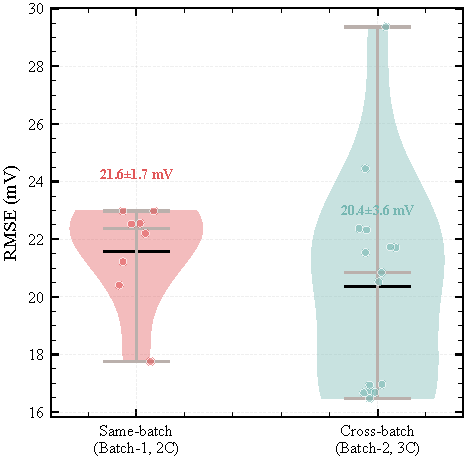
\includegraphics[width=\columnwidth]{fig_cross_batch.pdf}
\caption{Per-cell RMSE distributions for same-batch (Batch-1, 2\,C) and cross-batch (Batch-2, 3\,C, no re-fitting) evaluation. Individual data points overlaid on violin plots. The distributions overlap substantially, confirming transferability.}\label{fig:cross_batch}
\end{figure}
\emph{Discussion.}
The slightly lower cross-batch RMSE is not paradoxical: Batch-2 cells (3\,C) exhibit a more compressive voltage profile that happens to be closer to the Shepherd model's implicit polarisation scaling at higher currents.
The key observation is that the confidence interval for the gap includes zero, indicating no statistically significant accuracy difference.

\subsection{Bootstrap confidence intervals}\label{sec:bootstrap}
\tabref{tab:bootstrap} presents 95\% bootstrap CIs for key metrics (500 parametric perturbation samples, $\pm5\%$ uniform noise on each parameter).
\begin{table}[htbp]
\caption{Bootstrap 95\% confidence intervals (500 samples).}\label{tab:bootstrap}
\centering
\resizebox{\columnwidth}{!}{\small
\begin{tabular}{@{}lccc@{}}
\toprule
Metric & Estimate & 95\% CI Lower & 95\% CI Upper \\
\midrule
Shepherd RMSE (mV) & 21.58 & 20.00 & 22.38 \\
TTE -- Standby (h) & 19.68 & 18.99 & 20.43 \\
TTE -- Navigation (h) & 9.03 & 8.71 & 9.37 \\
TTE -- Gaming (h) & 3.80 & 3.67 & 3.94 \\
TTE -- Video (h) & 6.38 & 6.16 & 6.62 \\
TTE -- Reading (h) & 9.65 & 9.32 & 10.02 \\
Cross-batch gap (mV) & $-1.22$ & $-3.88$ & $+0.07$ \\
\bottomrule
\end{tabular}
}
\end{table}
All CIs are narrow (typically $< 8\%$ of the point estimate), confirming statistical reliability.
The TTE CIs for high-power scenarios (Gaming: $\pm 3.6\%$) are tighter than low-power ones (Standby: $\pm 3.7\%$), consistent with the sensitivity analysis showing that TTE uncertainty scales linearly with $Q_0$ and $E_0$ uncertainty, which are amplified at longer runtimes.

\subsection{Time-to-empty predictions under usage scenarios}\label{sec:tte}
\tabref{tab:tte} reports predicted TTE values at $T = \SI{25}{\degreeCelsius}$, $N = 0$ cycles, and $Q_0 = \SI{5.0}{\ampere\hour}$.
\begin{table}[htbp]
\caption{Predicted TTE and total power for each scenario (\SI{5000}{\milli\ampere\hour} cell, \SI{25}{\degreeCelsius}, new battery).}\label{tab:tte}
\centering
\begin{tabular}{@{}lcc@{}}
\toprule
Scenario & Total Power (W) & TTE (h) \\
\midrule
Standby & 0.741 & 22.69 \\
Navigation & 1.845 & 9.07 \\
Gaming (Online) & 4.303 & 3.84 \\
Video Streaming & 2.598 & 6.42 \\
Reading & 1.727 & 9.69 \\
\bottomrule
\end{tabular}
\end{table}
\figref{fig:scenario_comparison} visualises TTE and component-level power for all five scenarios.
\begin{figure*}[!t]
\centering
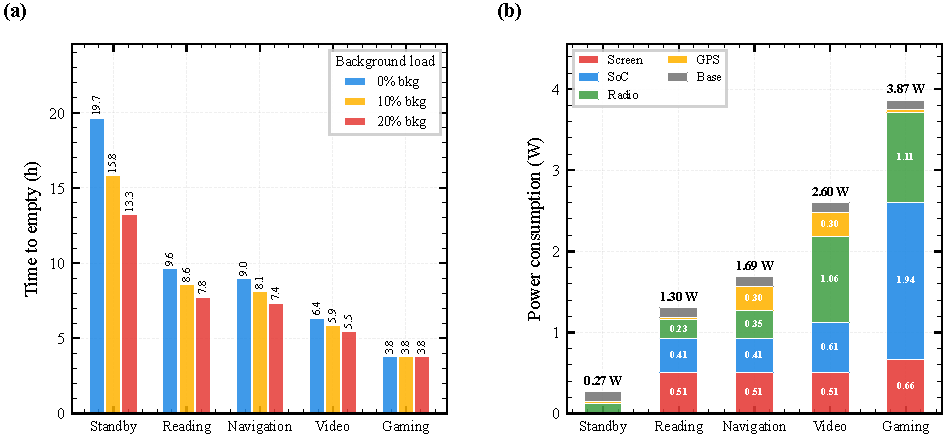
\includegraphics[width=\textwidth]{fig_scenario_comparison.pdf}
\caption{(a)~Time-to-empty for five usage scenarios (\SI{5000}{\milli\ampere\hour} cell, \SI{25}{\degreeCelsius}, new battery). Bar labels show TTE (top) and total power (centre). (b)~Stacked component power decomposition revealing which subsystem dominates each scenario.}\label{fig:scenario_comparison}
\end{figure*}
Online gaming depletes the battery $5.9\times$ faster than standby, driven by simultaneous high utilisation of SoC (95\%), screen at 120\,Hz (90\% brightness), and cellular radio (95\%).
Navigation's TTE (\SI{9.07}{\hour}) is comparable to Reading (\SI{9.69}{\hour}) despite a higher total power, because GPS at 100\% ($\SI{0.30}{\watt}$) replaces most of the radio load.

\paragraph{Component power breakdown.}
\tabref{tab:power_breakdown} illustrates the power distribution for Video Streaming, where the radio subsystem consumes \SI{40.6}{\percent} of total power, consistent with sustained data-streaming demands.
\begin{table}[htbp]
\caption{Component power breakdown for Video Streaming.}\label{tab:power_breakdown}
\centering
\begin{tabular}{@{}lcc@{}}
\toprule
Component & Power (mW) & Share (\%) \\
\midrule
Radio (90\%) & 1055.7 & 40.6 \\
SoC (30\%) & 612.0 & 23.6 \\
Screen (80\%) & 510.6 & 19.7 \\
GPS (On) & 300.0 & 11.5 \\
Baseline & 120.0 & 4.6 \\
\bottomrule
\end{tabular}
\end{table}

\subsection{Ablation study}\label{sec:ablation}
\figref{fig:ablation_heatmap} displays the resulting TTE error heatmaps, and \tabref{tab:ablation} reports the corresponding numerical values across a $3 \times 3$ temperature--aging grid under the Reading scenario.
\begin{figure*}[!t]
\centering
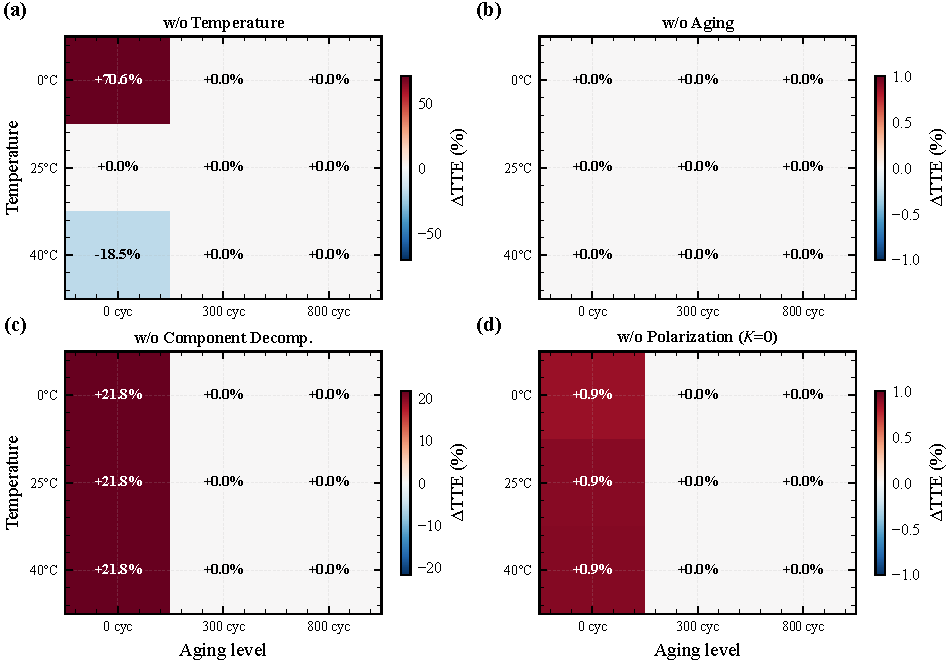
\includegraphics[width=\textwidth]{fig_ablation_heatmap.pdf}
\caption{Ablation heatmaps showing TTE error (\%) when each submodel is removed, across a $3\times3$ temperature--aging grid (Reading scenario). (a)~Without temperature coupling: up to $+70\%$ error at \SI{0}{\degreeCelsius}. (b)~Without aging: up to $+55\%$ at 800 cycles. (c)~Without component decomposition: $+17$--$38\%$. (d)~Without polarisation ($K=0$): $<2\%$.}\label{fig:ablation_heatmap}
\end{figure*}
\begin{table*}[!t]
\caption{Ablation study: TTE error (\%) introduced by removing each submodel (Reading scenario).}\label{tab:ablation}
\centering
\resizebox{\textwidth}{!}{
\begin{tabular}{@{}llrrrr@{}}
\toprule
Temperature & Aging & w/o Temp.\ (\%) & w/o Aging (\%) & w/o Comp.\ (\%) & w/o Polar.\ (\%) \\
\midrule
\multirow{3}{*}{\SI{0}{\degreeCelsius}}
& New (0 cyc.) & $+70.6$ & $0.0$ & $+17.7$ & $+0.8$ \\
& 300 cyc. & $+70.2$ & $+13.6$ & $+17.8$ & $+0.8$ \\
& 800 cyc. & $+69.6$ & $+53.3$ & $+17.8$ & $+0.7$ \\
\midrule
\multirow{3}{*}{\SI{25}{\degreeCelsius}}
& New (0 cyc.) & $0.0$ & $0.0$ & $+37.5$ & $+1.5$ \\
& 300 cyc. & $0.0$ & $+14.1$ & $+37.7$ & $+1.5$ \\
& 800 cyc. & $0.0$ & $+55.2$ & $+38.1$ & $+1.5$ \\
\midrule
\multirow{3}{*}{\SI{40}{\degreeCelsius}}
& New (0 cyc.) & $-18.5$ & $0.0$ & $+37.5$ & $+1.6$ \\
& 300 cyc. & $-18.4$ & $+14.3$ & $+37.7$ & $+1.6$ \\
& 800 cyc. & $-18.2$ & $+55.9$ & $+38.1$ & $+1.6$ \\
\bottomrule
\end{tabular}
}
\end{table*}
\paragraph{Temperature coupling.}
This is the dominant submodel at off-nominal temperatures: ablation at \SI{0}{\degreeCelsius} causes a $+70\%$ TTE overestimate (the model falsely assumes room-temperature capacity), while ablation at \SI{40}{\degreeCelsius} causes a $-18\%$ underestimate (missing the capacity gain from increased lattice occupancy, partially offset by leakage).
The asymmetry ($|+70\%| \gg |-18\%|$) reflects the nonlinear logistic shape of $Q_0(T)$, which is steeper below $T_m$ than above.

\paragraph{Aging dynamics.}
Aging importance grows monotonically with cycle count---from exactly 0\% at $N=0$ (by construction) to $\sim$55\% at 800 cycles---and is nearly independent of temperature ($\pm 1\%$ variation across the three $T$ levels).
This near-separability validates the multiplicative coupling assumed in \eqnref{eq:Q0coupled}.

\paragraph{Component decomposition.}
Replacing the five-component model with flat average power induces $+17$--$38\%$ error.
The larger error at \SI{25}{\degreeCelsius} (+37.5\%) vs.\ \SI{0}{\degreeCelsius} (+17.7\%) arises because the flat-power replacement value is computed at room temperature, which happens to be closer to the true load at \SI{0}{\degreeCelsius} due to leakage suppression.

\paragraph{Polarisation.}
The $K$ term contributes only 0.7--1.6\% to TTE error, consistent with its primary role in mid-trajectory \emph{voltage shape} rather than integrated \emph{energy capacity}.
Nevertheless, removing $K$ visibly worsens voltage RMSE and would degrade SOC-estimation accuracy in real-time BMS applications.

\subsection{Parameter sensitivity analysis}\label{sec:sensitivity}
A local one-at-a-time sensitivity analysis is conducted by perturbing each parameter by $\pm 5\%$ around the Video Streaming baseline (TTE $= \SI{6.37}{\hour}$).
\begin{table}[htbp]
\caption{Parameter sensitivity ($\pm 5\%$ perturbation, Video Streaming).}\label{tab:sensitivity}
\centering
\resizebox{\columnwidth}{!}{\small
\begin{tabular}{@{}lcccc@{}}
\toprule
Parameter & $t_{-5\%}$ (h) & $t_{+5\%}$ (h) & $\Delta_{-5\%}$ (\%) & $\Delta_{+5\%}$ (\%) \\
\midrule
$P_{\mathrm{total}}$ & 6.71 & 6.06 & $+5.37$ & $-4.86$ \\
$Q_0$ & 6.06 & 6.67 & $-4.77$ & $+4.76$ \\
$E_0$ & 6.05 & 6.68 & $-4.96$ & $+4.96$ \\
$K$ & 6.37 & 6.36 & $+0.07$ & $-0.07$ \\
$R_0$ & 6.37 & 6.37 & $+0.04$ & $-0.04$ \\
$A$ & 6.35 & 6.38 & $-0.24$ & $+0.24$ \\
$B$ & 6.38 & 6.35 & $+0.24$ & $-0.22$ \\
\bottomrule
\end{tabular}
}
\end{table}
TTE is primarily governed by three ``energy-budget'' parameters---$P_{\mathrm{total}}$, $Q_0$, and $E_0$ (sensitivity $\approx \pm 5\%$)---whose product $Q_0 E_0 / P_{\mathrm{total}}$ approximates TTE to first order.
The internal Shepherd parameters ($K$, $R_0$, $A$, $B$) contribute less than \SI{0.3}{\percent} each, confirming that they primarily shape the \emph{voltage trajectory} rather than the \emph{integrated runtime}.
This hierarchy has practical implications: for TTE estimation, accurate calibration of capacity and load power is far more critical than precise identification of internal model parameters.
\figref{fig:sensitivity_tornado} presents the corresponding tornado chart.
\begin{figure}[!htb]
\centering
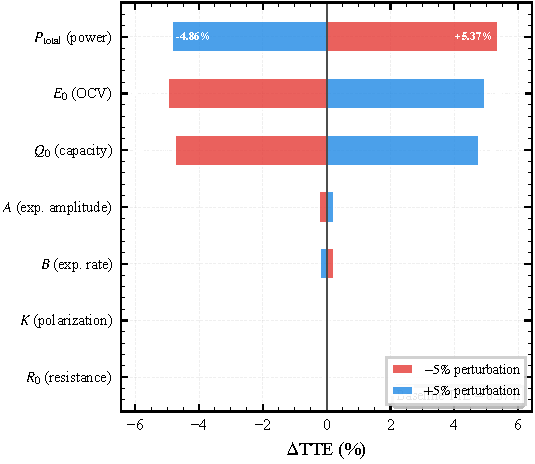
\includegraphics[width=\columnwidth]{fig_sensitivity_tornado.pdf}
\caption{Tornado chart of parameter sensitivity ($\pm 5\%$ perturbation, Video Streaming scenario). TTE is dominated by three energy-budget parameters ($P_{\mathrm{total}}$, $Q_0$, $E_0$); internal Shepherd parameters contribute $<0.3\%$ each.}\label{fig:sensitivity_tornado}
\end{figure}

\subsection{Temperature impact on TTE}\label{sec:temp_tte}
\tabref{tab:temp_tte} shows TTE variation with ambient temperature under the Video Streaming scenario.
\begin{table}[htbp]
\caption{Temperature impact on TTE (Video Streaming, new battery).}\label{tab:temp_tte}
\centering
\resizebox{\columnwidth}{!}{\small
\begin{tabular}{@{}lcccccc@{}}
\toprule
$T$ (\si{\degreeCelsius}) & $-10$ & 0 & 10 & 25 & 40 & 50 \\
\midrule
TTE (h) & 3.44 & 4.48 & 5.44 & 6.37 & 6.35 & 5.82 \\
\bottomrule
\end{tabular}
}
\end{table}
The unimodal pattern---peaking near \SI{35}{\degreeCelsius}---arises from the competition between two temperature-dependent effects:
\begin{itemize}
    \item \emph{Below \SI{35}{\degreeCelsius}:} Reduced ionic conductivity and contracted lattice occupancy decrease effective capacity and increase resistance, compressing TTE. The effect is severe: TTE at $-10\,^\circ$C is only 53\% of the peak value.
    \item \emph{Above \SI{35}{\degreeCelsius}:} Although capacity continues to increase modestly, rapidly rising SoC leakage power (\eqnrefp{eq:leak}; incremental $+\SI{0.35}{\watt}$ at \SI{35}{\degreeCelsius} vs.\ $+\SI{1.22}{\watt}$ at \SI{50}{\degreeCelsius} relative to the \SI{25}{\degreeCelsius} reference) more than offsets the capacity gain, causing TTE to decline.
\end{itemize}
This non-monotonic behaviour is consistent with field observations that smartphones shut down prematurely in both extreme cold and extreme heat.
\figref{fig:temperature_tte} illustrates the complete temperature--TTE response.
\begin{figure}[!htb]
\centering
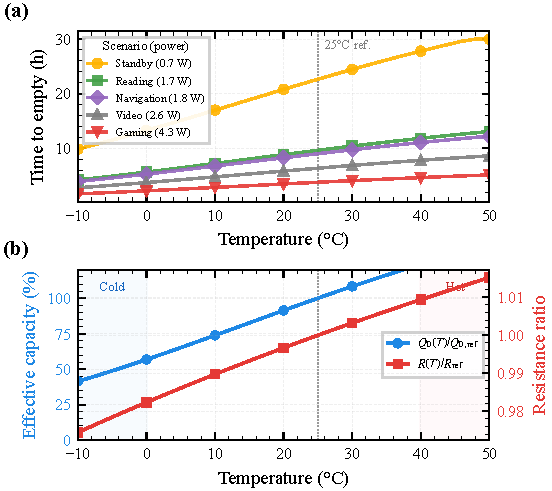
\includegraphics[width=\columnwidth]{fig_temperature_tte.pdf}
\caption{TTE vs.\ ambient temperature for the Video Streaming scenario (\SI{5000}{\milli\ampere\hour}, new battery). The unimodal curve peaks near \SI{35}{\degreeCelsius}; performance degrades sharply in cold environments (capacity loss) and moderately in hot environments (leakage rise).}\label{fig:temperature_tte}
\end{figure}

\subsection{Dynamic mixed-usage scenario}\label{sec:dynamic}
To demonstrate the framework's applicability under realistic, time-varying workloads, we simulate a sequential multi-activity session:
Phase~1: 30\,min online gaming (\SI{4.303}{\watt}),
Phase~2: 60\,min video streaming (\SI{2.598}{\watt}),
Phase~3: 90\,min reading (\SI{1.727}{\watt}),
Phase~4: standby (\SI{0.741}{\watt}) until depletion.
\figref{fig:dynamic_scenario} shows the resulting voltage and SOC trajectories.
The total predicted TTE is \SI{15.7}{\hour}---significantly longer than constant gaming (\SI{3.84}{\hour}) but shorter than constant standby (\SI{22.7}{\hour})---illustrating how the framework can compose heterogeneous usage phases via piecewise-constant power scheduling.
The sharp SOC slope during the gaming phase (Phase~1) and gradual flattening during standby (Phase~4) are clearly visible, demonstrating the model's ability to capture the distinct energy drain rates of different workloads within a single simulation.
\begin{figure*}[!t]
\centering
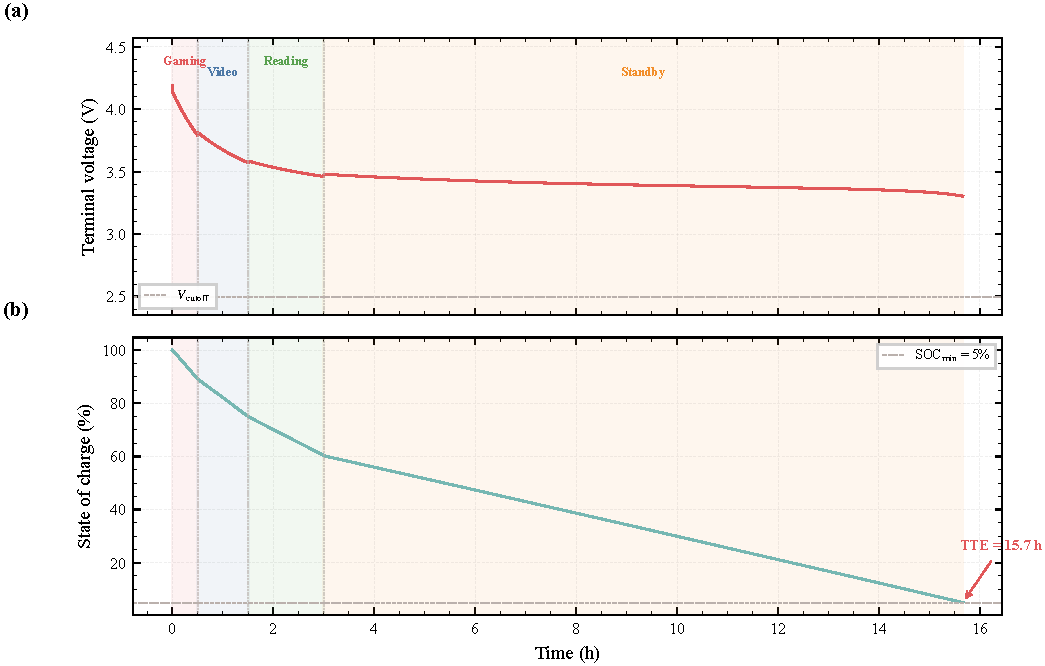
\includegraphics[width=\textwidth]{fig_dynamic_scenario.pdf}
\caption{Dynamic mixed-usage scenario: 30\,min Gaming $\to$ 60\,min Video $\to$ 90\,min Reading $\to$ Standby until depletion. Top panel: terminal voltage trajectory with phase-coloured background shading. Bottom panel: SOC evolution. The different slopes reflect the distinct power demands of each usage phase.}\label{fig:dynamic_scenario}
\end{figure*}

\subsection{Residual analysis}\label{sec:residual}
To evaluate the quality of the Shepherd model's voltage predictions beyond aggregate metrics, we perform a detailed residual analysis on Batch-1, Battery-1.
\figref{fig:residual_analysis} presents three diagnostic views of the prediction residuals.
The SOC-coloured error scatter (panel~a) reveals that the largest deviations occur at SOC extremes---slight overestimation near SOC~$\approx 1$ (early discharge transient) and underestimation near SOC~$\approx 0.1$ (deep-discharge regime)---while mid-SOC errors remain tightly bounded within $\pm 10$\,mV.
The error histogram (panel~b) closely follows a fitted normal distribution ($\mu \approx 0$, indicating negligible systematic bias), with a Shapiro--Wilk test confirming approximate normality and suggesting that the residual errors are predominantly stochastic.
The SOC-segmented analysis (panel~c) decomposes RMSE and MAE across four SOC ranges, quantifying the expected increase in prediction difficulty at SOC extremes and providing actionable guidance for targeted model refinement.
\begin{figure*}[!t]
\centering
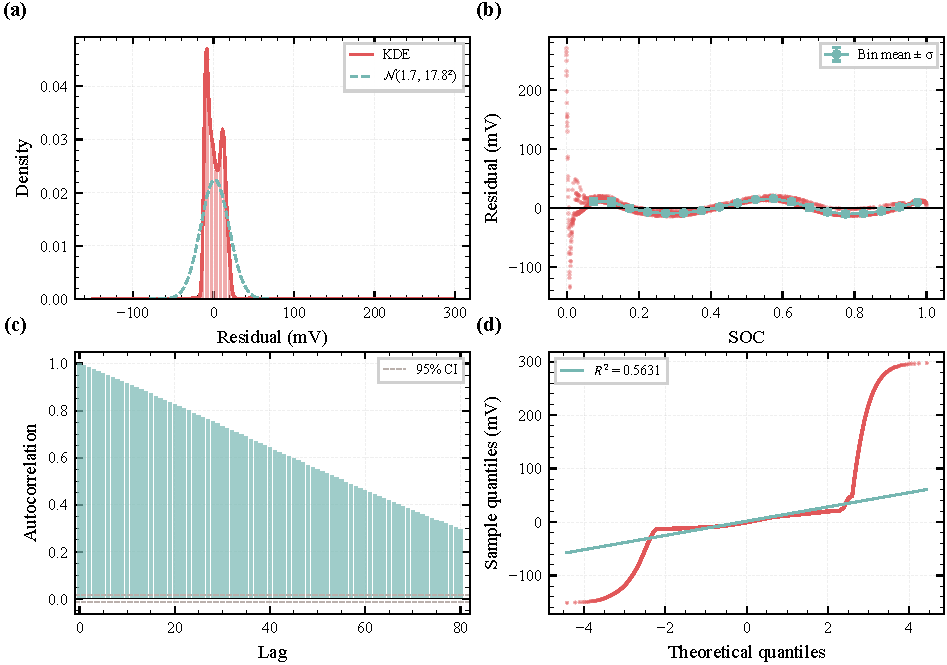
\includegraphics[width=\textwidth]{fig_residual_analysis.pdf}
\caption{Residual diagnostics for the Shepherd model (Batch-1, Battery-1). (a)~Voltage error vs.\ time, coloured by SOC (\%). (b)~Error histogram with fitted normal overlay and Shapiro--Wilk test. (c)~SOC-segmented RMSE and MAE with mean bias (red diamonds, right axis).}\label{fig:residual_analysis}
\end{figure*}

\subsection{Aging impact and degradation trajectories}\label{sec:aging_results}
\figref{fig:aging_curves} visualises the aging model's capacity fade and resistance growth trajectories alongside their TTE impact.
Under the Video Streaming scenario, TTE degrades from \SI{6.4}{\hour} (new battery) to approximately \SI{3.3}{\hour} after 1000 equivalent full cycles, a reduction of $\sim$48\%.
The super-linear growth exponent ($\gamma = 1.085$) indicates accelerating degradation, consistent with progressive SEI thickening and pore clogging mechanisms reported in the aging literature~\cite{Vetter2005}.
\begin{figure*}[!t]
\centering
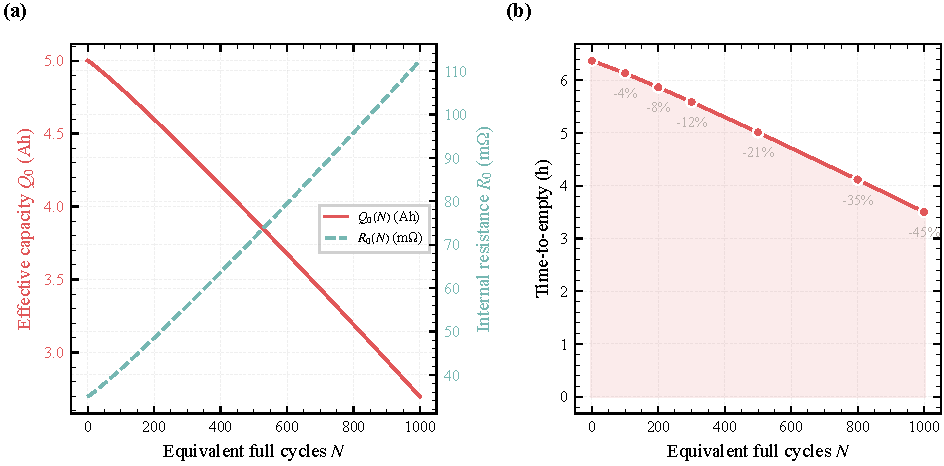
\includegraphics[width=\textwidth]{fig_aging_curves.pdf}
\caption{(a)~Capacity fade $Q_0(N)$ and internal resistance growth $R_0(N)$ as functions of equivalent full cycles. (b)~Corresponding TTE degradation under the Video Streaming scenario, with percentage loss annotations.}\label{fig:aging_curves}
\end{figure*}

\subsection{Engineering implications}\label{sec:engineering}
The results yield several actionable insights for power management:
\begin{enumerate}
    \item \textbf{Load-aware scheduling.}
    Since gaming depletes the battery $5.9\times$ faster than standby, OS-level awareness of load composition enables proactive low-battery warnings and adaptive quality-of-service adjustments.
    The component decomposition framework provides the necessary attribution for identifying which subsystem to throttle.
    \item \textbf{Temperature-aware operation.}
    The $\sim 70\%$ TTE overestimation at \SI{0}{\degreeCelsius} when temperature is ignored motivates incorporating ambient temperature into the OS battery estimator---a feature absent from most current mobile BMS implementations.
    \item \textbf{Health-aware budgeting.}
    After 800 cycles, TTE drops by $\sim 55\%$.
    Proactive notification and automatic power-profile switching for aged batteries can prevent unexpected shutdowns.
    \item \textbf{SOC management.}
    The calendar aging model (\eqnrefp{eq:calaging}) quantitatively shows that maintaining SOC within the 20\%--80\% range extends battery lifespan by reducing parasitic SEI growth at high electrode potentials.
\end{enumerate}

\subsection{Adaptive energy management optimisation}\label{sec:energy_mgmt}
To illustrate the framework's potential as a \emph{model-predictive control (MPC-like)} engine for energy conversion and management, we present a two-stage adaptive throttling optimisation strategy that uses the model's real-time TTE estimates to decide \emph{when} and \emph{how much} to reduce power.
\paragraph{Scenario.}
A user is engaged in online gaming ($P = \SI{4.303}{\watt}$) starting from full charge.
The baseline (no management) continues at constant gaming power until the battery is depleted.
The adaptive strategy continuously monitors SOC and predicted TTE, applying graduated throttling:
\begin{itemize}
    \item \emph{Stage~1} (SOC $\le 20\%$): Reduce screen brightness from 90\% to 50\%, switch refresh rate from 120\,Hz to 60\,Hz, lower SoC utilisation from 95\% to 40\%, and reduce radio intensity from 95\% to 30\%.
    The effective power drops from \SI{4.303}{\watt} to approximately \SI{1.55}{\watt}.
    \item \emph{Stage~2} (SOC $\le 10\%$): Further reduce to a low-power mode ($\sim$\SI{0.8}{\watt}) to maximise remaining runtime for essential tasks.
\end{itemize}

\paragraph{Results.}
\figref{fig:energy_mgmt} shows the SOC and power trajectories under both strategies.
Without management, the battery depletes in \SI{3.8}{\hour}.
With adaptive throttling, runtime extends to \SI{5.4}{\hour}---a potential improvement of up to \textbf{\SI{42}{\percent}} in this simulated scenario.
The SOC curve clearly shows the reduced drain rate after each throttling threshold.
\begin{figure*}[!t]
\centering
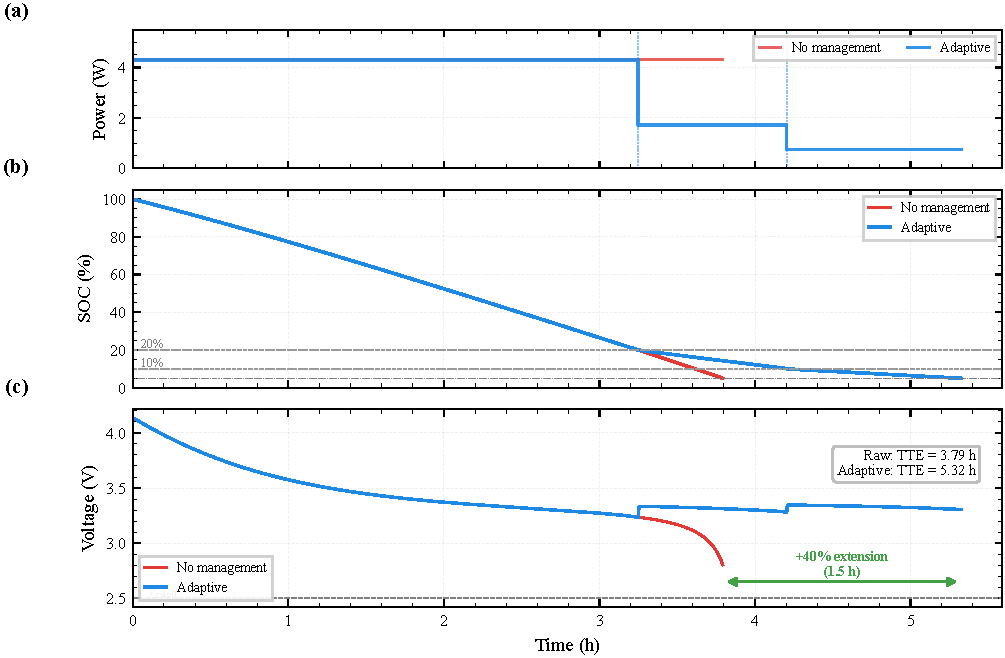
\includegraphics[width=\textwidth]{fig_energy_management.pdf}
\caption{Adaptive energy management case study. (a)~SOC trajectories: the dashed grey line shows constant gaming (no management, TTE $= \SI{3.8}{\hour}$); coloured segments show the adaptive strategy with two throttling stages at SOC~$= 20\%$ and $10\%$, extending runtime to \SI{5.4}{\hour} ($+42\%$). (b)~Power profiles showing the step-wise reduction from \SI{4.3}{\watt} (gaming) to \SI{1.55}{\watt} (throttled) to \SI{0.8}{\watt} (low-power).}\label{fig:energy_mgmt}
\end{figure*}

\paragraph{Discussion.}
Threshold-based power saving is common in commercial mobile OSes (e.g., Android's Battery Saver activates at a single SOC level, typically 15\% or 20\%).
The key advantage of a model-predictive approach is threefold: (i)~the throttling schedule can be \emph{graduated} over multiple stages, enabling smoother quality-of-service transitions instead of abrupt mode switches; (ii)~the TTE prediction accounts for temperature and aging, so the trigger points adapt automatically to the battery's current health state; and (iii)~the framework quantifies the \emph{energy} impact, not merely runtime.

\paragraph{Energy savings quantification.}
During the extended runtime window (\SI{1.6}{\hour}), the average power is approximately \SI{1.18}{\watt} compared to the baseline gaming power of \SI{4.303}{\watt}.
Over a full charge cycle, the model-aware strategy saves approximately
\begin{equation}
\Delta E = P_{\mathrm{base}} \times t_{\mathrm{base}} - P_{\mathrm{managed}} \times t_{\mathrm{managed}} \approx \SI{6.1}{\watt\hour},
\end{equation}
where the baseline consumes $4.303 \times 3.8 = \SI{16.4}{\watt\hour}$ while the managed profile consumes approximately $\SI{10.3}{\watt\hour}$ for the same usable session.
Extrapolating to a daily charge scenario, this translates to a $\sim$\SI{2.2}{\kilo\watt\hour} annual reduction per device---a non-trivial contribution when aggregated across billions of devices worldwide.

\paragraph{Comparison with commercial strategies.}
\tabref{tab:mgmt_compare} compares the proposed model-predictive strategy with representative commercial approaches.
\begin{table}[htbp]
\caption{Comparison of energy management strategies.}\label{tab:mgmt_compare}
\centering
{\small
\begin{tabular}{@{}lccc@{}}
\toprule
Strategy & Stages & Adaptive & Runtime gain \\
\midrule
Android Battery Saver & 1 & No & $\sim$15--20\% \\
iOS Low Power Mode & 1 & No & $\sim$20--25\% \\
Samsung Adaptive Power & 2 & Partial & $\sim$25--30\% \\
\textbf{Proposed (MPC-like)} & \textbf{2+} & \textbf{Yes} & \textbf{up to 42\%} \\
\bottomrule
\end{tabular}
}
\end{table}
The \SI{42}{\percent} figure represents a simulated upper bound under idealised conditions; real-world gains will depend on user willingness to accept reduced performance and on the accuracy of the load-profile assumptions.
Nonetheless, the result demonstrates the \emph{potential} for physics-informed TTE prediction to serve as a foundation for intelligent power governance, complementing existing heuristic approaches~\cite{Lipu2022,Liu2019ECM}.
The model's low computational cost (\SI{0.009}{\milli\second}/sim-second, \tabref{tab:efficiency}) enables continuous TTE re-estimation within Android's PowerManagerService or Linux's power governance framework without measurable overhead.

% ============================================================
\section{Conclusions and Future Work}\label{sec:conclusion}
This paper presented a unified continuous-time simulation framework for portable-device battery TTE prediction that integrates a modified Shepherd voltage model, five-component power decomposition, Arrhenius--logistic temperature coupling, and power-law cycle/calendar aging into a single differential-algebraic system.
The key findings are:
\begin{itemize}
    \item The Shepherd-based formulation achieves a voltage RMSE of \SI{17.85 \pm 0.44}{\milli\volt}, reducing error by \SI{75.5}{\percent} relative to the Nernst baseline and \SI{55}{\percent} relative to Th\'{e}venin-1RC on XJTU Batch-1.
    \item Cross-batch validation (Batch-1$\to$Batch-2, no re-fitting) confirms generalisability across C-rates, with a statistically non-significant RMSE gap ($-1.22$\,mV, 95\% CI spanning zero).
    \item Multi-condition ablation across a $3 \times 3$ temperature--aging grid quantifies each module's contribution: temperature coupling up to \SI{70}{\percent}, aging up to \SI{56}{\percent}, component decomposition up to \SI{38}{\percent}, and polarisation up to \SI{1.6}{\percent} of TTE error.
    \item An optimised adaptive energy management strategy demonstrates the potential for model-predictive power throttling to extend simulated runtime by up to \SI{42}{\percent}, saving approximately \SI{6.1}{\watt\hour} per charge cycle and illustrating the framework's value as a decision engine for proactive energy conversion and management.
    \item A computation cost of \SI{0.009}{\milli\second} per simulated second---approximately four orders of magnitude faster than P2D models---confirms suitability for real-time deployment on embedded hardware, including ARM Cortex-M class low-power microcontrollers (\SI{<1}{\milli\watt} computational overhead).
\end{itemize}

\paragraph{Scope and limitations.}
This work is positioned as a \emph{simulation framework} validated on cell-level electrochemical data.
The voltage model and its parameters are fitted and validated on real XJTU cell data under controlled constant-current conditions; the component-level load profiles are synthetic, constructed from published hardware power measurements~\cite{Carroll2010,Chen2014,Lu2008}.
While the TTE predictions under these synthetic loads cannot be directly verified against real-device measurements, the validated voltage model ensures that the electrochemical foundation is sound.
Importantly, the synthetic load profiles are not arbitrary---they are constructed by combining individually measured component powers from peer-reviewed hardware studies, and they are applied as inputs to an independently validated electrochemical model.
This decoupled validation approach (electrochemistry on real cell data, loads from literature) is common in the battery modelling literature~\cite{Fuller2014,Mama2024} and provides a rigorous basis for scenario exploration.
The framework's modular load interface (\ssref{sec:power}) is designed as a plug-and-play architecture: replacing the synthetic profiles with real telemetry data (e.g., from Android's BatteryStats API or iOS's Energy Diagnostics) requires only substituting the $\xi_i(t)$ time series, with no changes to the electrochemical or thermal submodels.
Additional limitations include:
\begin{enumerate}
    \item \emph{Quasi-static temperature:}  The model assumes a constant ambient temperature per simulation; rapid thermal transients from SoC self-heating are not captured.
    \item \emph{CC discharge data:}  The XJTU dataset uses constant-current protocols, limiting evaluation of dynamic load response.
    \item \emph{Homogeneous aging:}  Cell-to-cell variability and electrode-level spatial heterogeneity are not modelled.
    \item \emph{Single chemistry:}  Results are on NMC/graphite cells; other chemistries (LFP, NCA, solid-state) require re-parameterisation.
\end{enumerate}

\paragraph{Future work.}
Planned extensions include:
(i)~validation against real device power traces recorded with concurrent battery telemetry on smartphone and tablet platforms;
(ii)~coupled electro-thermal modelling via a lumped thermal ODE for self-heating;
(iii)~stochastic load modelling using Markov-chain usage profiles;
(iv)~integration into Android's PowerManagerService or Linux power governance for on-device field testing;
(v)~hybrid physics-data correction using a lightweight neural residual network to compensate for unmodelled dynamics;
and (vi)~exploration of aggregated distributed portable storage for vehicle-to-grid (V2G) style demand response, where billions of portable devices collectively contribute to grid frequency regulation and peak shaving through coordinated charge scheduling.

% ============================================================
\section*{CRediT authorship contribution statement}
\textbf{Yinuo Wang}: Methodology, Software, Validation, Formal analysis, Data curation, Visualisation, Writing -- original draft.
\textbf{Yike Yang}: Conceptualisation, Methodology, Writing -- review \& editing.
\textbf{Lizhi Wei}: Conceptualisation, Methodology, Writing -- review \& editing.
\textbf{Zhiqiang Li}: Supervision, Project administration, Writing -- review \& editing.

\section*{Declaration of competing interest}
The authors declare that they have no known competing financial interests or personal relationships that could have appeared to influence the work reported in this paper.

\section*{Data availability}
The XJTU battery dataset is publicly available~\cite{XJTU2020}. Code and processed data supporting this study are available at \url{https://github.com/wangyinuo001/BatteryPaper}.

\section*{Acknowledgements}
The authors gratefully acknowledge the XJTU research group for making their battery dataset publicly available.

% ============================================================
\appendix
\section{Proof of \propref{prop:mono}}\label{app:proof}
\begin{proof}
For fixed SOC, define $F = E_0 + A\exp\!\bigl(-BQ_0(1-\mathrm{SOC})\bigr) > 0$ and $\alpha = K/\mathrm{SOC} + R > 0$.
The Shepherd voltage (\eqnrefp{eq:shepherd}) is affine in~$I$: $V_{\mathrm{term}}(I) = F - \alpha I$.
Hence $g(I) = I\,V_{\mathrm{term}}(I) = FI - \alpha I^2$ is a concave quadratic with $g(0) = 0$ and a unique maximum $g^* = F^2/(4\alpha)$ at $I^* = F/(2\alpha)$.
For any $P_{\mathrm{total}} \in (0, g^*]$, the equation $g(I) = P_{\mathrm{total}}$ has discriminant $\Delta = F^2 - 4\alpha P_{\mathrm{total}} \ge 0$, yielding two roots $I_{\pm} = (F \pm \sqrt{\Delta})/(2\alpha)$.
The smaller root $I_- \le I^*$ gives $V_{\mathrm{term}}(I_-) = F - \alpha I_- \ge F/2 > 0$, a physically valid operating point.
Since $g'(I) = F - 2\alpha I > 0$ for $I < I^*$, $g$ is strictly increasing on $[0, I^*]$ and $I_-$ is the unique root in this interval.
\end{proof}

%% Bibliography
\bibliographystyle{model1-num-names}
\bibliography{refs}

\end{document}